\section{Auswertung}
\label{sec:Auswertung}
Die Messwerte für den Winkel $\phi$ des Prismas sind in Tabelle \ref{tab:phimess} aufgetragen.
\begin{table}[H]
    \caption{Messwerte der $\phi$-Messung.}
    \label{tab:phimess}
    \centering
    \begin{tabular}{S[table-format=3.1(0)e0] 
					S[table-format=3.1(0)e0] 
					S[table-format=2.2(0)e0] }
        \toprule
        {$\phi_r/\si{\degree}$} &
        {$\phi_l/\si{\degree}$} &
        {$\phi/\si{\degree}$}  \\
		\midrule
139.3   & 259.4  & 60.05	\\
142.4   & 262.4  & 60.0	\\
136.6   & 256.4  & 59.9	\\
143.4   & 263.3  & 59.95	\\
138.6   & 258.5  & 59.95	\\
146.0   & 266.0  & 60.0	\\
140.6   & 260.4  & 59.9	\\
		\bottomrule
    \end{tabular}
\end{table}
\noindent
Es ergibt sich somit ein mittlerer Winkel von:
\begin{equation}
	\overline\phi = \SI{59.96\pm0.02}{\degree}
\end{equation}
Die Messwerte der $\eta$-Messung sind in Tabelle \ref{tab:etamess} aufgetragen. Zusätzlich sind die Wellenlängen der beobachteten Spektrallinien\cite{cd}\cite{hg} aufgetragen.
\begin{table}[H]
    \caption{Messwerte der $\eta$-Messung.}
    \label{tab:etamess}
    \centering
    \begin{tabular}{S[table-format=3.1(0)e0] 
					S[table-format=2.1(0)e0] 
					S[table-format=3(0)e0] 
					S[table-format=2.1(0)e0] }
        \toprule
        {$\Omega_r/\si{\degree}$} &
        {$\Omega_l/\si{\degree}$} &
        {$\lambda/\si{\nano\meter}$}  &
        {$\eta/\si{\degree}$} \\
		\midrule
207.4   & 89.6   & 644  & 62.2\\
206.7   & 90.1   & 577  & 63.4\\
206.4   & 90.5   & 546  & 64.1\\
205.9   & 91.0   & 509  & 65.1\\
205.4   & 91.4   & 480  & 66.0\\
205.1   & 91.7   & 468  & 66.6\\
204.3   & 92.5   & 436  & 68.2\\
203.3   & 93.4   & 405  & 70.1\\
		\bottomrule
    \end{tabular}
\end{table}
\noindent
Der Winkel $\eta$ berechnet sich gemäß Gleichung \eqref{eq:eta}.
Die Gleichung \eqref{eq:snell} kann auf die folgende Form gebracht werden:
\begin{equation}
	n = \frac{\sin{\frac{\eta+\phi}{2}}}{\sin{\frac{\phi}{2}}}
\end{equation}
Es ergeben sich folgende Wertepaare $(n_i, \lambda_i)$:
\begin{table}[H]
    \caption{Messwerte der $\eta$-Messung.}
    \label{tab:nl}
    \centering
    \begin{tabular}{S[table-format=1.4(6)e0] 
					S[table-format=3.0(0)e0] }
        \toprule
        {$n$}  &
        {$\lambda/\si{\nano\meter}$}  \\
		\midrule
1.7516\pm0.0004         & 644\\
1.7616\pm0.0004         & 577\\
1.7674\pm0.0004         & 546\\
1.7755\pm0.0004         & 509\\
1.7827\pm0.0004         & 480\\
1.7874\pm0.0004         & 468\\
1.7998\pm0.0004         & 436\\
1.8141\pm0.0004         & 405\\
		\bottomrule
    \end{tabular}
\end{table}
\noindent
Diese Wertepaare können nun auf zwei verschiedene Möglichkeiten genähert werden, wie in Gleichung \eqref{eq:f1} oder so wie in Gleichung \eqref{eq:f2}.
Für beide Funktionen werden die Parameter mittels Python/SciPy optimiert und im Diagramm \ref{fig:dis} aufgetragen.
\begin{figure}[H]
  \centering
  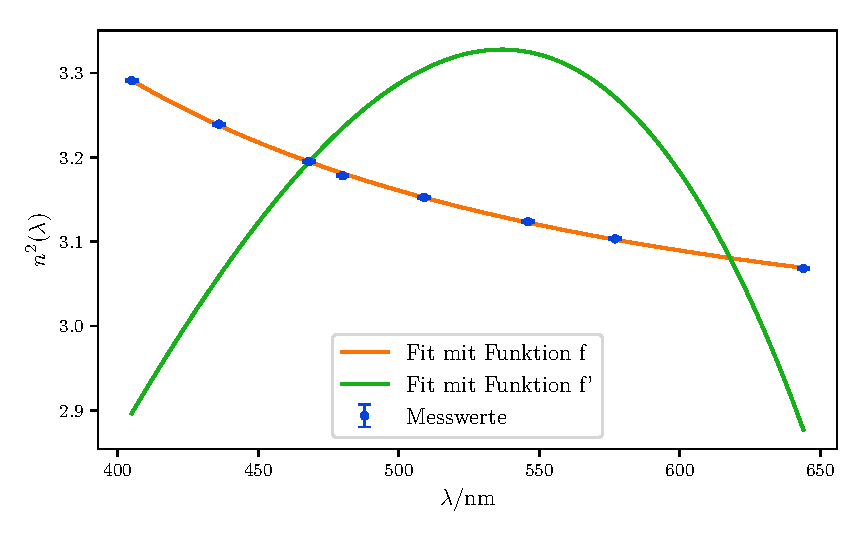
\includegraphics[width=\textwidth]{build/n.pdf}
  \caption{Dispersionskurven aus den zwei verschiedenen Ansätzen \eqref{eq:f1} und \eqref{eq:f2}.}
  \label{fig:dis}
\end{figure}
\noindent
Die Parameter ergeben sich zu:
\begin{align}
	A_0 =& \SI{2.921\pm0.002}{} \\
	A_2 =& \SI{6.02\pm0.04e4}{\per\nano\meter\squared} \\
%	A_2 =& \SI{1.25\pm0.39e9}{\per\nano\meter\tothe{4}} \\
\nonumber \\
	A_0' =& \SI{3.386\pm0.002}{} \\
	A_2' =& \SI{8.25\pm0.06e-7}{\per\nano\meter\squared} \\
%	A_4' =& \SI{2.81\pm0.01e-11}{\per\nano\meter\tothe{4}} 
\end{align}
Die Summe der Abweichungsquadrate wird gemäß
\begin{equation}
	s^2 = \frac{1}{N-2}\sum_i^N\left(n^2(\lambda_i) - f(\lambda_i)\right)^2
\end{equation}
bestimmt.
Es ergeben sich folgende Werte:
\begin{align}
	s^2 =& \num{6.08\pm0.08e-6} \\
	{s'}^2 =& \num{5.77\pm0.04e-4} 
\end{align}
Im Folgenden wird deshalb nur die Vorschrift aus Gleichung \eqref{eq:f1} verwendet.
Aus der Herleitung von Gleichung \eqref{eq:f1} erkennt man, dass
\begin{align}
	A_0 =& \alpha + 1 \\
	A_2 =& \alpha\lambda_1^2 \\
	\lambda_1 =& \sqrt{\frac{A_2}{A_0 - 1}} 
\end{align}
gelten muss,
wobei die unphysikalischen Lösungen $\lambda_1 = 0$ und $\lambda_1 < 0$ außer Acht gelassen werden.
Es folgt:
\begin{align}
	\lambda_1 =& \SI{177.0\pm0.7}{\nano\meter} \\
\end{align}
Die Unsicherheit ergibt sich aus:
\begin{equation}
	\symup\Delta\lambda_1 = \sqrt{\left(\sqrt{\frac{A_2}{A_0-1}}\frac{\symup\Delta A_2}{2A_2}\right)^2 + \left(\left(\frac{A_2}{A_0-1}\right)^\frac{3}{2}\frac{\symup\Delta A_0}{2A_2}\right)^2 }
\end{equation}
Die Abbesche Zahl, ein Maß für die Farbzersteruung, berechnet sich wie folgt:
\begin{equation}
	\nu = \frac{n(\SI{589}{\nano\meter})-1}{n(\SI{486}{\nano\meter})-n(\SI{656}{\nano\meter})}
\end{equation}
Die Unsicherheit ist hierbei:
\begin{equation}
	\symup\Delta\nu = \sqrt{
		\left( \frac{\symup\Delta n(\SI{589}{\nano\meter})}{n(\SI{486}{\nano\meter})-n(\SI{656}{\nano\meter})} \right)^2 +
		\left( \frac{(n(\SI{589}{\nano\meter})-1)(\symup\Delta n(\SI{486}{\nano\meter})+\symup\Delta n(\SI{656}{\nano\meter}))}{(n(\SI{486}{\nano\meter})-n(\SI{656}{\nano\meter}))^2)}\right)^2}
\end{equation}
Wobei gegeben ist:
\begin{equation}
	\symup\Delta n(\lambda) = \sqrt{{\symup\Delta A_0}^2 + \left(\frac{\symup\Delta A_2}{\lambda^2}\right)^2}
\end{equation}
Mit der zuvor bestimmten Dispersionsfunktion ergibt sich ein Wert von:
\begin{equation}
	\nu = \num{18.23\pm0.13}
\end{equation}
Das Auflösungsvermögen gibt an, wie nah zwei Wellenlängen sich sein dürfen, damit sie immernoch unterscheidbar sind.
Es ist definiert durch
\begin{equation}
	A := \frac{\lambda}{\symup\Delta\lambda} = b\left\lvert\frac{\symup dn}{\symup{d\lambda}}\right\rvert = b\left\lvert\frac{2A_2}{\lambda^3}\right\rvert,
\end{equation}
wobei $b=\SI{3}{\centi\meter}$\cite{v402} die Basislänge des Prismas darstellt.
Die Unsicherheit lässt sich bestimmen nach:
\begin{equation}
	\symup\Delta A = b\left\lvert\frac{2\symup\Delta A_2}{\lambda^3}\right\rvert
\end{equation}
Es ergeben sich beispielhaft Werte für $A$ von:
\begin{align}
	A(\SI{656}{\nano\meter}) =& \num{1.28\pm0.01e4} \\ 
	A(\SI{486}{\nano\meter}) =& \num{3.15\pm0.02e4} 
\end{align}
